%% ------------------------------------------------------------------------- %%
\chapter{Resultados}
\label{cap:resultados}

Os resultados obtidos através do processamento metodológico serão enumerados a
aseguir.


%% ------------------------------------------------------------------------- %%
\section{Resultados Anteriores}\index{área do trabalho!fundamentos}
\label{sec:fundamentos}

Texto texto texto texto texto texto texto texto texto texto texto texto texto
texto texto texto texto texto texto texto texto texto texto texto texto texto
texto texto texto texto texto texto texto texto texto texto texto texto texto


%% ------------------------------------------------------------------------- %%
\subsection{GSHAP}\index{área do trabalho!fundamentos}
\label{sec:fundamentos}

Texto texto texto texto texto texto texto texto texto texto texto texto texto
texto texto texto texto texto texto texto texto texto texto texto texto texto
texto texto texto texto texto texto texto texto texto texto texto texto texto



%% ------------------------------------------------------------------------- %%
\subsection{Zoneamento Sísmico}\index{área do trabalho!fundamentos}
\label{sec:fundamentos}

Texto texto texto texto texto texto texto texto texto texto texto texto texto
texto texto texto texto texto texto texto texto texto texto texto texto texto
texto texto texto texto texto texto texto texto texto texto texto texto texto

Cornell \& McGuire !?!?


%% ------------------------------------------------------------------------- %%
\subsubsection{Dourado, 2014}\index{área do trabalho!fundamentos}
\label{sec:fundamentos}


Na Figura~\ref{fig:dour_h_c} a ameaça sísmica calculada com o programa
Crisis-v2007.

\begin{figure}[!h]
  \centering
  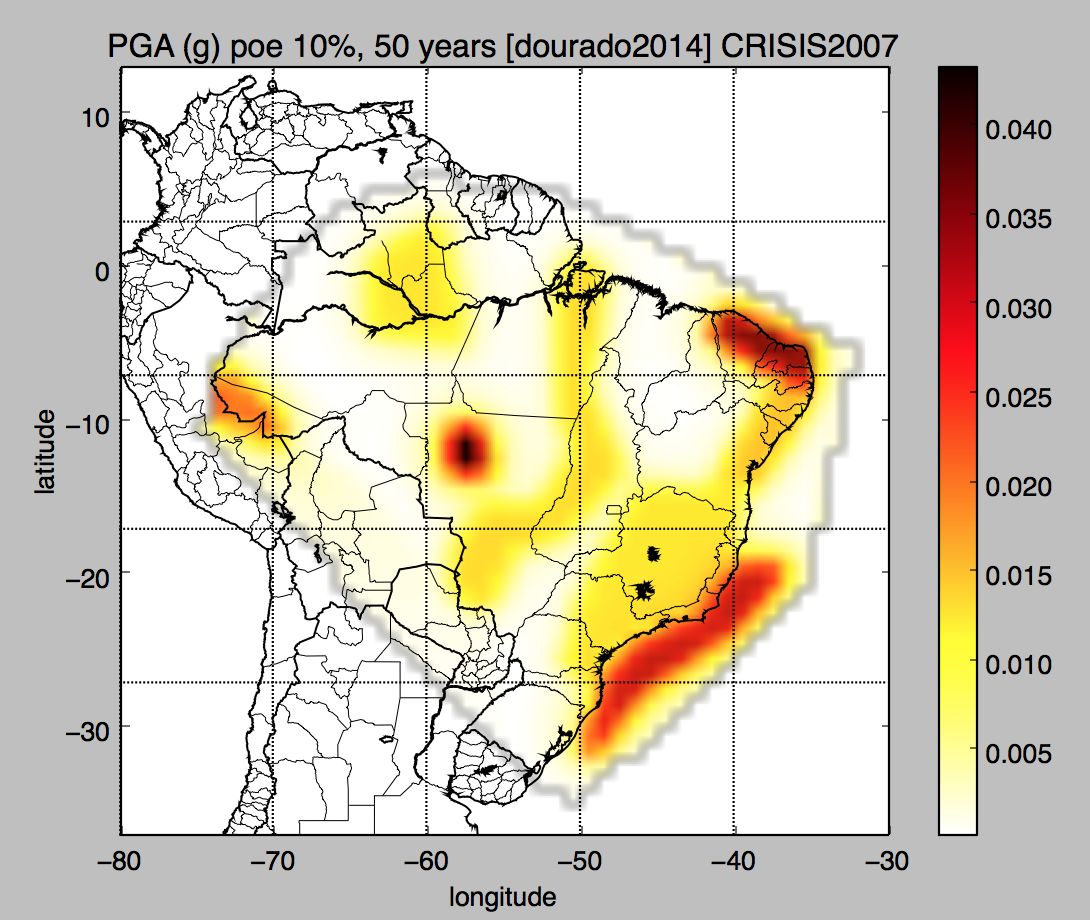
\includegraphics[width=.80\textwidth]{dour_h_c} 
  \caption{Seismic Rate: a(m > $M_{min}$ = 0) [Dourado, 2014, Crisis-2007] }
  \label{fig:dour_h_c} 
\end{figure}

Os valores em gal $[cm/s^2]$) foram convertidos para unidades de \emph{g}
$[m/s^2]$.


Na Figura~\ref{fig:dour_h_o} é apresentado o resultado do zoneamento sísmico
feito por Dourado, 2014, calculado com o oq-engine.

\begin{figure}[!h]
  \centering
  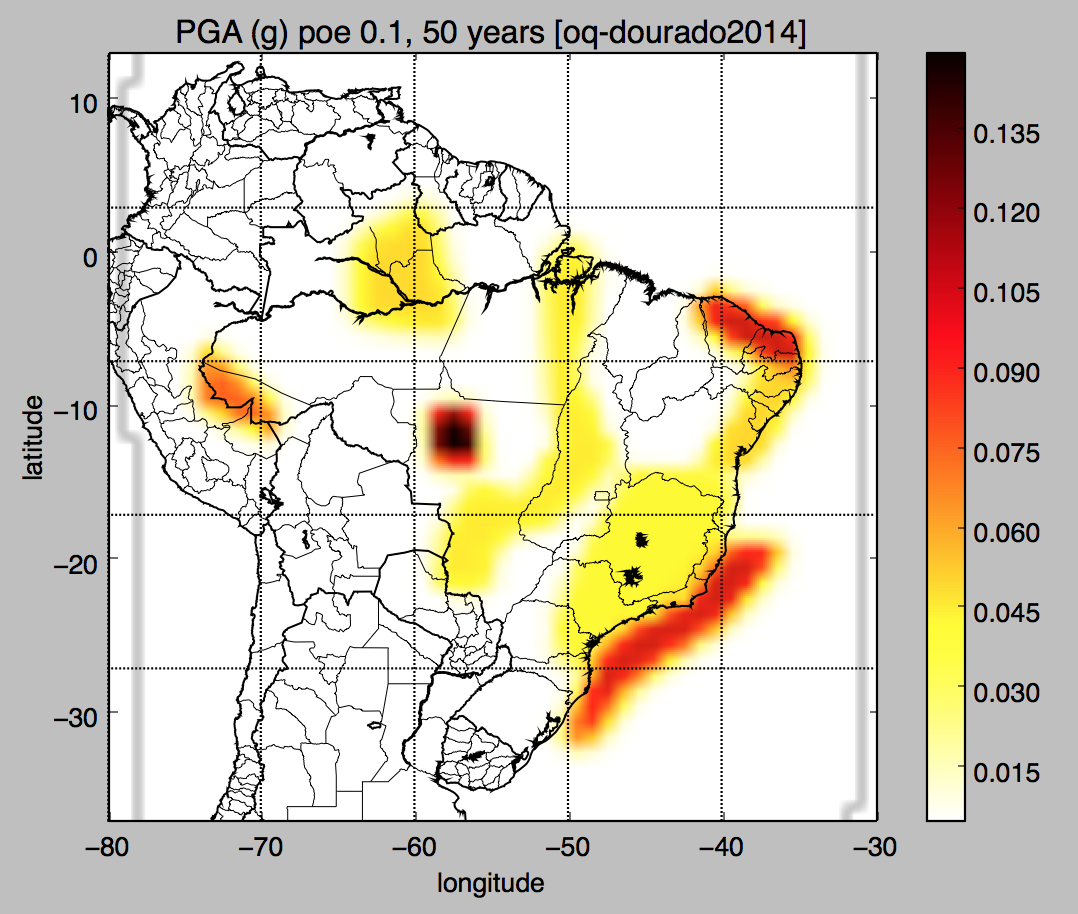
\includegraphics[width=.80\textwidth]{dour_h_o} 
  \caption{Seismic Hazard: PGA(poe 0.1, 50y)[Dourado, 20014] OpenQuake-Engine }
  \label{fig:dour_h_o} 
\end{figure}


Podemos observar que\ldots


%% ------------------------------------------------------------------------- %%
\section{Suavização da Sismicidade}\index{área do trabalho!fundamentos}
\label{sec:fundamentos}

Dentre os métodos de suavização que foram investigados, são apresentados os
seguintes resultados.

bla bla bla bla bla bal.
bla bla bla bla bla bal.
bla bla bla bla bla bal.
bla bla bla bla bla bal.
bla bla bla bla bla bal.
bla bla bla bla bla bal.



%% ------------------------------------------------------------------------- %%
\subsection{Frankel, 1995}\index{área do trabalho!fundamentos}
\label{sec:fundamentos}

bla bla bla bla bla bal.
bla bla bla bla bla bal.
bla bla bla bla bla bal.
bla bla bla bla bla bal.
bla bla bla bla bla bal.
bla bla bla bla bla bal.



O médodo de suavização proposto por Frankel, 1995, resultou na seguinte taxa de
sismicidade observada na figura \ref{fig:fran_r}.

\begin{figure}[!h]
  \centering
  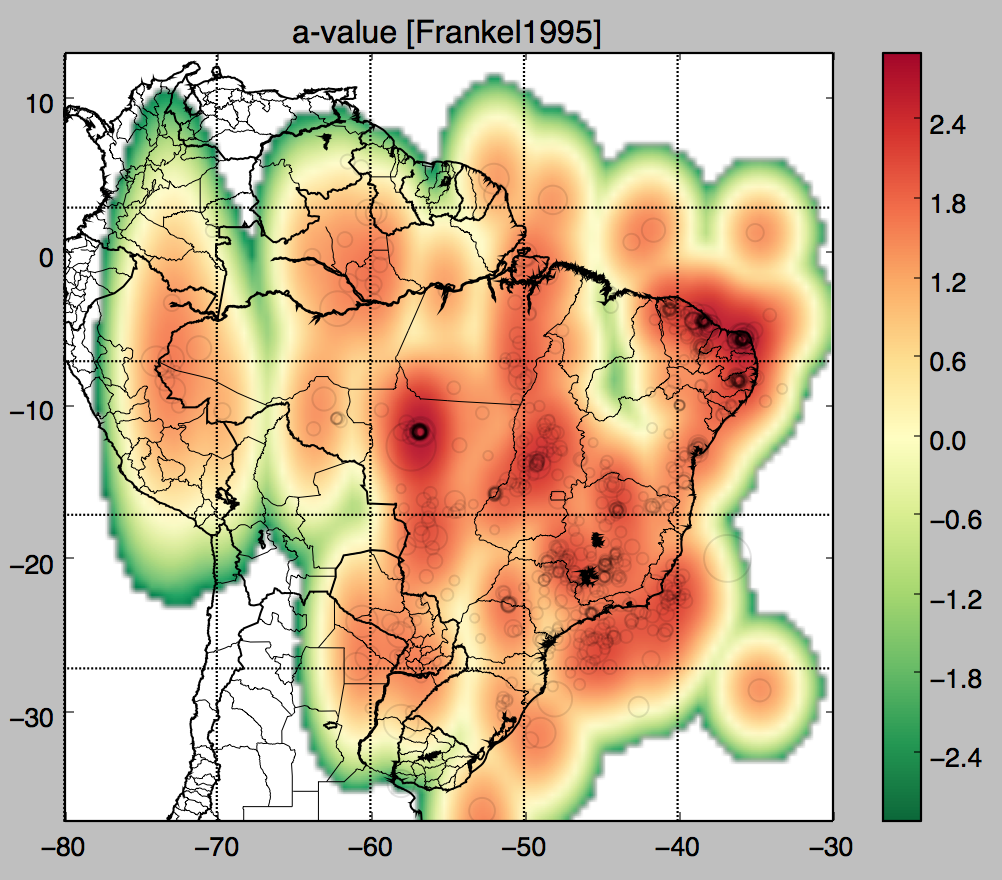
\includegraphics[width=.80\textwidth]{fran_r} 
  \caption{Seismic Rate: a(m > $M_{min}$ = 0) [Frankel, 1995] }
  \label{fig:fran_r} 
\end{figure}

Em seguida, na figura~\ref{fig:fran_h}, se pode observar os valores da ameaça
sísmica.

bla bla bla bla bla bal.
bla bla bla bla bla bal.
bla bla bla bla bla bal.
bla bla bla bla bla bal.
bla bla bla bla bla bal.
bla bla bla bla bla bal.



\begin{figure}[!h]
  \centering
  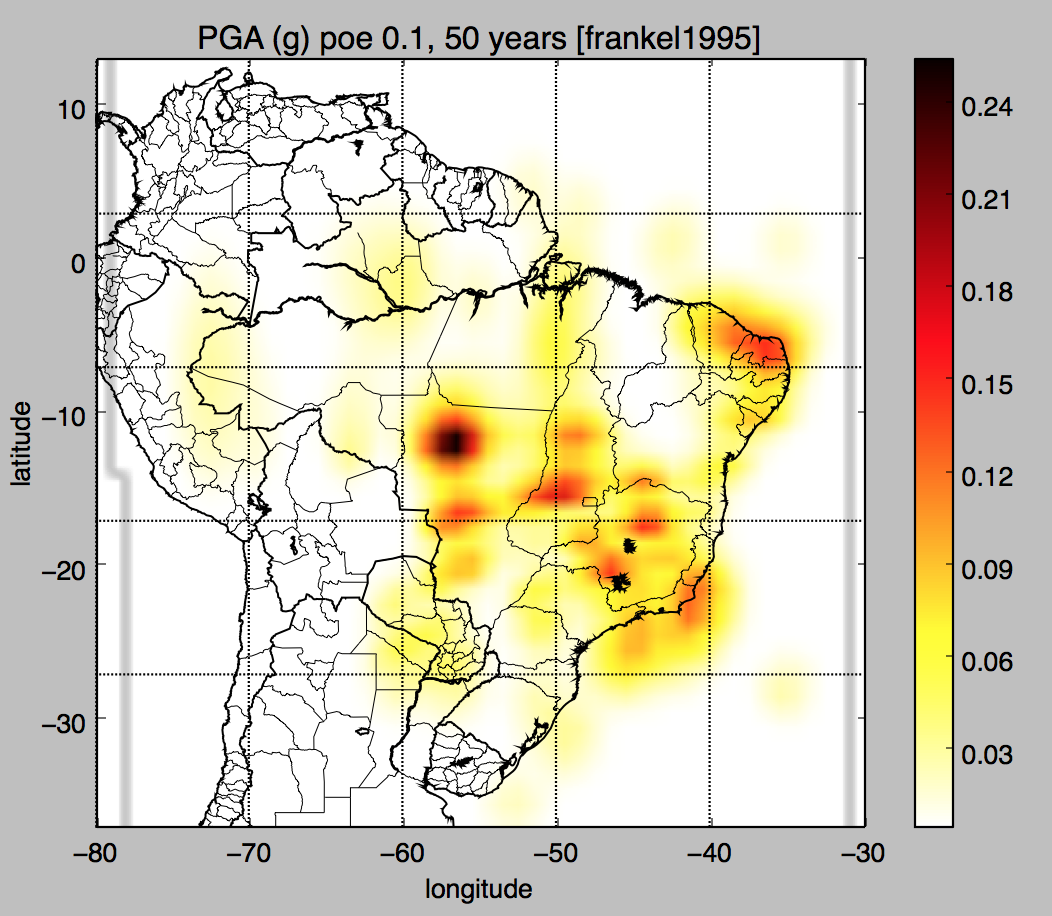
\includegraphics[width=.80\textwidth]{fran_h} 
  \caption{Seismic Hazard: PGA(poe 0.1, 50y)[Frankel, 1995] }
  \label{fig:fran_h} 
\end{figure}


Os resultados\ldots

bla bla bla bla bla bal.
bla bla bla bla bla bal.
bla bla bla bla bla bal.
bla bla bla bla bla bal.
bla bla bla bla bla bal.
bla bla bla bla bla bal.

%% ------------------------------------------------------------------------- %%
\subsection{Woo, 1996}\index{área do trabalho!fundamentos}
\label{sec:fundamentos}

bla bla bla bla bla bal.
bla bla bla bla bla bal.
bla bla bla bla bla bal.
bla bla bla bla bla bal.
bla bla bla bla bla bal.
bla bla bla bla bla bal.


Aplicando o método de Woo, na Figura~\ref{fig:woo_r} temos:

\begin{figure}[!h]
  \centering
  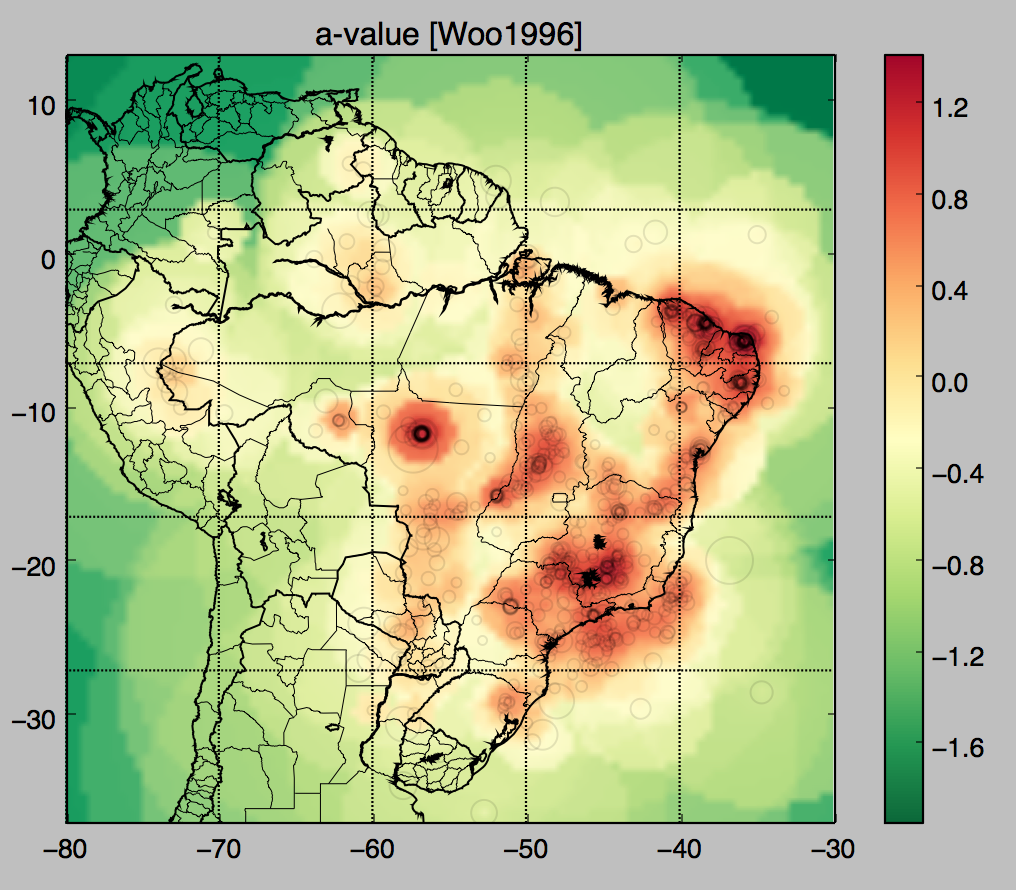
\includegraphics[width=.80\textwidth]{woo_r} 
  \caption{Seismic Rate: a(m > $M_{min}$ = 0) [Woo, 1996] }
  \label{fig:woo_r} 
\end{figure}

bla bla bla bla bla bal.
bla bla bla bla bla bal.
bla bla bla bla bla bal.
bla bla bla bla bla bal.
bla bla bla bla bla bal.
bla bla bla bla bla bal.

A ameaça pode ser vista na figura \ref{fig:woo_h}:

\begin{figure}[!h]
  \centering
  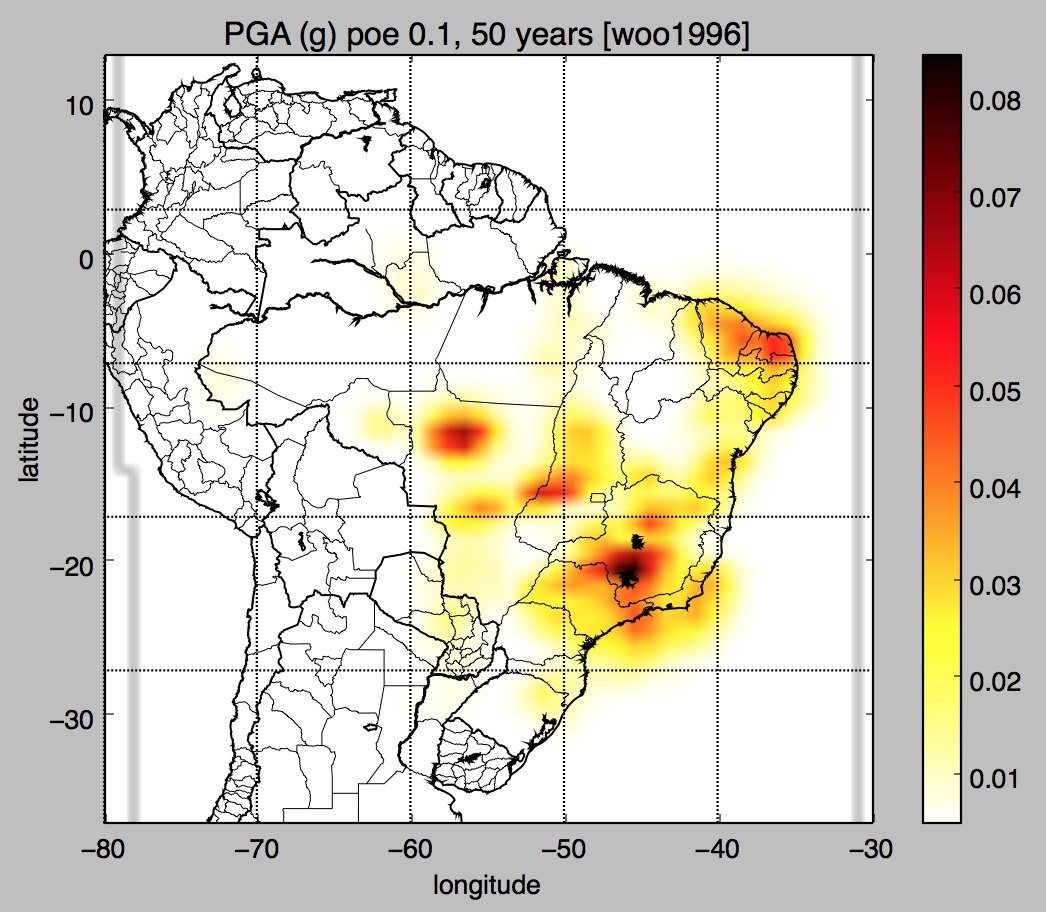
\includegraphics[width=.80\textwidth]{woo_h} 
  \caption{Seismic Hazard: PGA(poe 0.1, 50y)[Woo, 1996] }
  \label{fig:woo_h} 
\end{figure}


Podemos observar \ldots

bla bla bla bla bla bal.
bla bla bla bla bla bal.
bla bla bla bla bla bal.
bla bla bla bla bla bal.
bla bla bla bla bla bal.
bla bla bla bla bla bal.


%% ------------------------------------------------------------------------- %%
\subsection{Helmstetter, 2012}\index{área do trabalho!fundamentos}
\label{sec:fundamentos}

bla bla bla bla bla bal.
bla bla bla bla bla bal.
bla bla bla bla bla bal.
bla bla bla bla bla bal.
bla bla bla bla bla bal.
bla bla bla bla bla bal.

Usando o método proposto por Helmstetter para a taxa de sismicidade de
longo-prazo temos na figura \ref{fig:helm_r} a seguinte taxa de sismicidade:

\begin{figure}[!h]
  \centering
  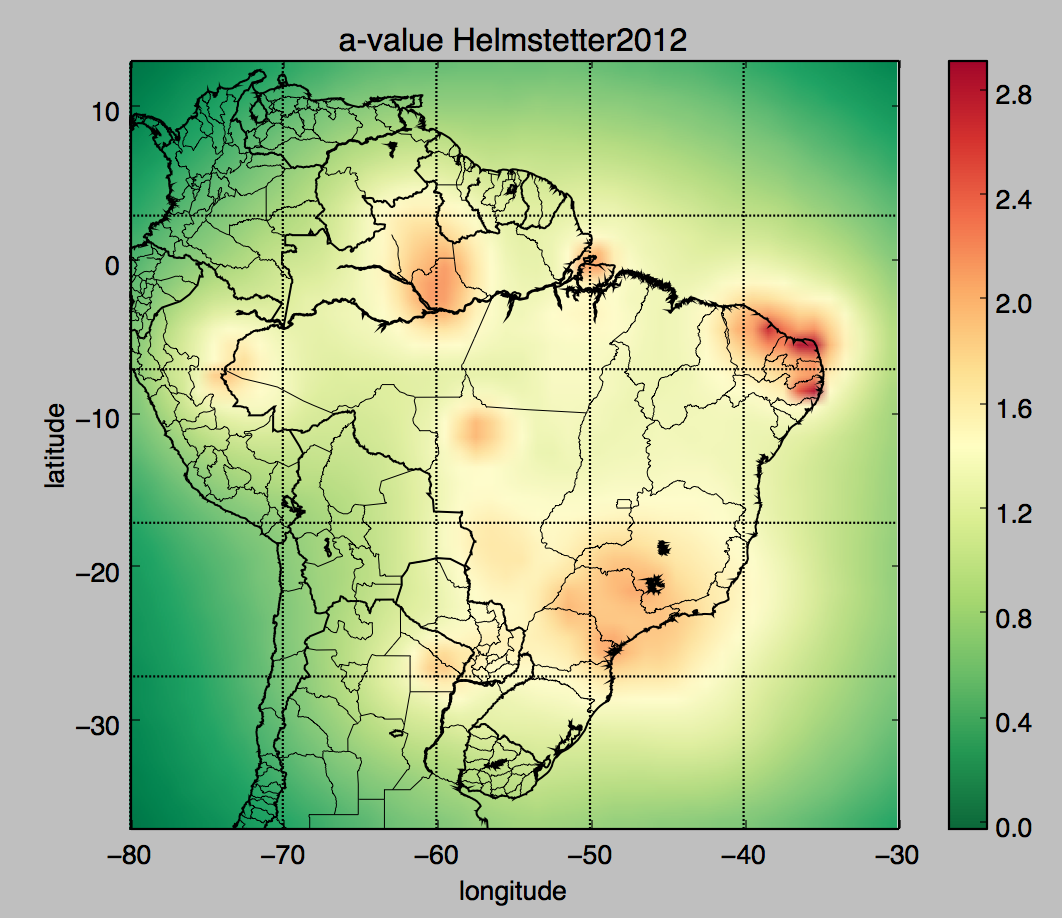
\includegraphics[width=.80\textwidth]{helm_r} 
  \caption{Seismic Rate: a(m > $M_{min}$ = 0) [Helmstetter, 2012] }
  \label{fig:helm_r} 
\end{figure}

bla bla bla bla bla bal.
bla bla bla bla bla bal.
bla bla bla bla bla bal.
bla bla bla bla bla bal.
bla bla bla bla bla bal.
bla bla bla bla bla bal.

E, na figura~\ref{fig:helm_h} o respectivo mapa de ameaça:

\begin{figure}[!h]
  \centering
  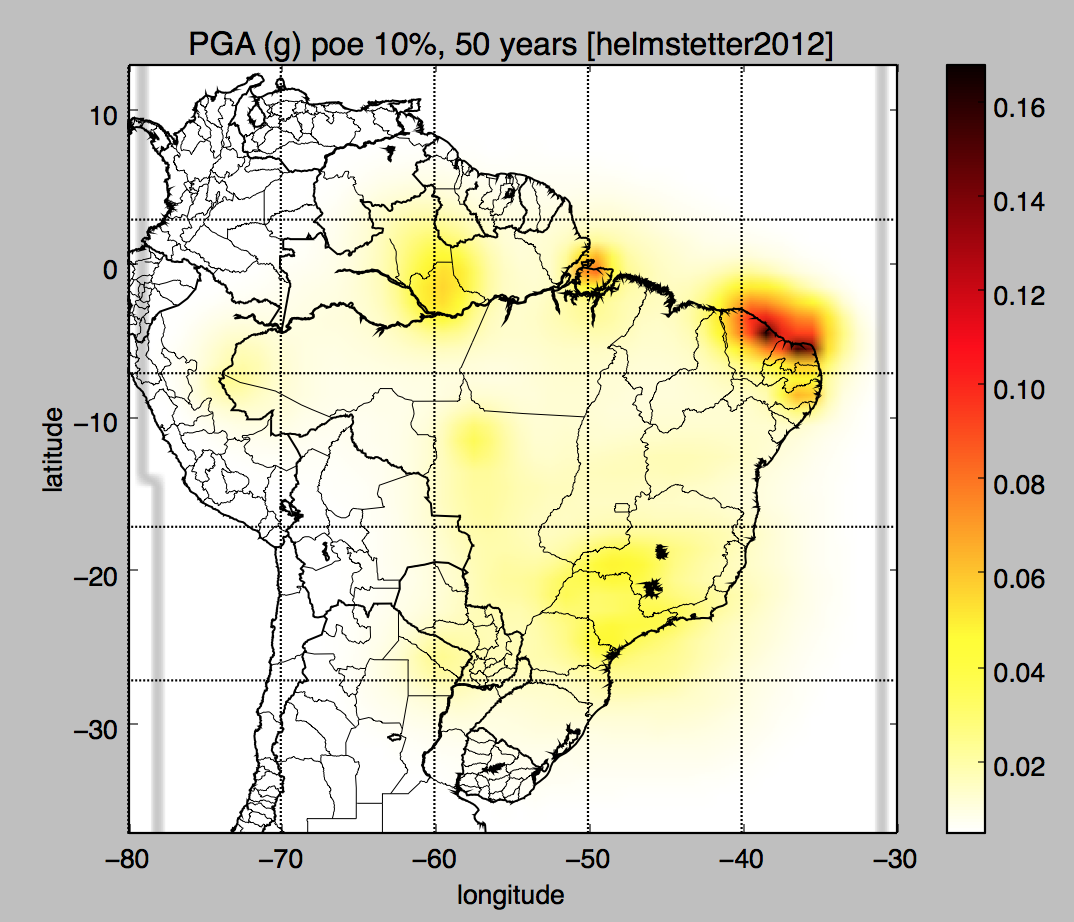
\includegraphics[width=.80\textwidth]{helm_h} 
  \caption{Seismic Hazard: PGA(poe 0.1, 50y)[Helmstetter2012] }
  \label{fig:helm_h} 
\end{figure}


Podemos observar que\ldots

